  Dieses Kapitel behandelt die Evaluation der Java Web Frameworks. Es wird die
  kombinierte Methode, aus gewichteter Nutzwertanalyse und \ac{AHP}, aus dem
  Kapitel \ref{chapter:MethodenZurEntscheidungsfindungBeiEinerEvaluation}
  \nameref{chapter:MethodenZurEntscheidungsfindungBeiEinerEvaluation} (auf
  Seite \pageref{chapter:MethodenZurEntscheidungsfindungBeiEinerEvaluation}ff)
  angewendet. Mit der Definition von sinnvollen Rahmenbedingungen, soll die
  Evaluation durchgeführt und das Resultate in Form einer Rangliste vorgelegt
  werden.
    
  \section{Rahmenbedingungen}
  
  Über Soll-Kriterien und KO-Kriterien werden die Rahmenbedingungen für die
  Evaluierung festgelegt. Die Soll-Kriterien widerspiegeln die Anforderungen,
  welche an ein Java Web Framework gestellt werden. Die KO-Kriterien dienen zum
  Ausschluss, nicht geeigneter Frameworks.

  \section{Auswahl der Java Web Frameworks}
  
  Es sollen vier Java Web Frameworks für die Evaluation ausgewählt werden. Ein
  Java Web Framework, das in Frage kommt, wird Alternative genannt. Jede
  Alternative wird mit einer ID in der Form \{A\}-\{Laufnummer\} versehen.
  
  \subsection{Begründung}
  
  Es soll für jede Alternative der Grund der Wahl erläutert werden. In
  Absprache\footnote{Siehe Anhang \ref{chapter:KickOffProtokoll}
  \nameref{chapter:KickOffProtokoll} S. \pageref{chapter:KickOffProtokoll} und
  \ref{chapter:DesignReviewProtokoll} \nameref{chapter:DesignReviewProtokoll}
  S. \pageref{chapter:DesignReviewProtokoll}} mit dem Projektbetreuer soll aus
  den verschiednen Gruppen von Java Web Frameworks jeweils eines gewählt werden.
  Es wurden folgende Typen definiert:
  
  \begin{itemize}
    \item \ac{RIA} - Frameworks
    \item MVC - Frameworks
    \item Java Script/HTML/CSS - Cross-Compiler Frameworks
    \item In der \ac{ZKB} bereits eingesetzte Frameworks
  \end{itemize}
  
  \subsubsection{A-1 - ULC, Canoo RIA Suite}
  
  ULC, Canoo RIA Suite zählt zu der Gruppe der \ac{RIA} Frameworks. Gemäss
  Kick-off Protokoll Beschluss\footnote{Siehe Anhang
  \ref{chapter:KickOffProtokoll} \nameref{chapter:KickOffProtokoll} S.
  \pageref{chapter:KickOffProtokoll}} soll dieses Framework als Alternative
  gewählt werden. Zudem wird die ULC, Canoo RIA Suite bereits von den Schweizer
  Banken Credit Suisse und UBS eingesetzt.
  
  \subsubsection{A-2 - Struts 1.3.10 mit ZIP-Framework}
  
  Struts 1.3.10 mit ZIP-Framework zählt zu der Gruppe der MVC - Frameworks. Es
  wird in der \ac{ZKB} bereits eingesetzt. Das Framework wird innerhalb der
  \ac{ZKB} für die Umsetzung der Online Bank verwendet und gilt als Standard
  für neue Projekte, siehe \cite{ZkbHandbuchDerItArchitektur}  S. 140. Damit
  das Ergebnis der Evaluation Begründet werden kann, sollte ein Vergleich mit
  diesem Framework existieren.
  
  \subsubsection{A-3 - Vaadin 6.6.0}
  
  Vaadin zählt zu der Gruppe der Java Script/\ac{HTML}/\ac{CSS} -
  Cross-Compiler Frameworks. Es baut auf \ac{GWT} auf, das in den letzten
  Jahren an Aufmerksamkeit gewonnen hat und auch im Finanzsektor eingesetzt
  wird, siehe \cite{GWTImFinanzSektor}. Vaadin wird auch in der Finanzbranche
  der Schweiz eingesetzte, so zählt zum Beispiel, die Betreiberin des
  Finanzmarks Schweiz, die SIX Group, zu dessen Anwender, siehe
  \cite{VaadinInDerSchweiz}.
  
  \subsubsection{A-4 - Apache Wicket 1.4.17}
  
  Apache Wicket gehört zu der Gruppe die in der ZKB bereits eingesetzt wird.
  Die Wahl ist auf Apache Wicket gefallen, da es sich schon länger am Markt
  etabliert hat und somit auf eine breite Community stützt. Die
  Einsatzfähigkeit innerhalb der Bank  hat es auch schon bewiesen.
  
  \section{Prüfen der zu beachtenden KO-Kriterien}
  
  Es soll eine Prüfung aller Java Web Frameworks statt finden, ob ein solches
  gegen definierte KO-Kriterien verstösst. Falls das der Fall ist, wird das
  Framework von der Evaluation ausgeschlossen. Falls das nicht zutrifft, wird
  das Framework in die Evaluation mit einbezogen, siehe Abbildung
  \ref{img:ablaufEvaluation}.
  
  In Absprache mit dem Fachbetreuer der \ac{ZKB} gibt es gewisse KO-Kriterien,
  die im Rahmen der Diplomarbeit ausser Kraft treten, und somit bei dieser
  Prüfung nicht beachtet werden sollen, siehe Abschnitt
  \ref{section:KoKriterienDieNichtBeachtetWerden}
  \nameref{section:KoKriterienDieNichtBeachtetWerden} (auf Seite
  \pageref{section:KoKriterienDieNichtBeachtetWerden}). Das Resultat wird in
  der Tabelle \ref{tab:gefundeneKOKriterien} dargestellt.
  \newline
  
  \begin{table}[!h]
    \sffamily 
    \begin{center}
      \begin{tabular}{lcc}
        \toprule
        \textbf{Java Web Framework} & \textbf{Verstoss gg KO-Kriterium} &
        \textbf{Ausschluss}\\
        \midrule
        A-1 - ULC, Canoo RIA Suite & \ref{itm:KO-18} & Ja\\
        & \ref{itm:KO-19} &\\
        A-2 - Struts 1.3.10 mit ZIP-Framework & - & Nein\\
        A-3 - Vaadin 6.6.0 & - & Nein\\
        A-4 - Apache Wicket 1.4.17 & - & Nein\\
        \bottomrule
      \end{tabular}
      \caption{Verstösse gegen KO-Kriterien}
      \label{tab:gefundeneKOKriterien}
    \end{center}
  \end{table}

  \subsection{A-1 - ULC, Canoo RIA Suite - KO-Kriterien gefunden}
  
  Leider wurde während der Analyse festgestellt, dass die ULC, Canoo RIA Suite
  nur in einer Java Virtual Machine\footnote{Die Java Virtual Machine ist der
  Teil der \ac{JRE}, der für die Ausführung des Java-Bytecodes verantwortlich
  ist, siehe \cite{JavaVirtualMachine}.} lauffähig ist. Das wird über die
  Technik von Java-Web-Start\footnote{Java-Web-Start ist eine Technik von
  Oracle (damals entwickelt von Sun Microsystems), die es ermöglicht, Java-Anwendungen
  über das Internet mit nur einem Klick zu starten. Im Unterschied zu
  Java-Applets benötigen Java-Web-Start-Anwendungen keinen Browser, um ablaufen
  zu können, siehe \cite{JavaWebStart}.} oder mit der Hilfe von einem
  Java-Applet\footnote{Ein Java-Applet ist ein Computerprogramm, das in der
  Programmiersprache Java verfasst wurde und normalerweise in einem Webbrowser
  ausgeführt wird, siehe \cite{JavaApplet}.} vollbracht. Das ist ersichtlich im
  ULC Architektur Guide, siehe \cite{ULCArchitectureGuide} S. 18. Damit
  verstösst diese Alternative gegen die KO-Kriterien \ref{itm:KO-18} und
  \ref{itm:KO-19}. Aufgrund des Vorgehens aus der Abbildung
  \ref{img:ablaufEvaluation} wird diese Alternative aus der Evaluation
  ausgeschlossen.
  
  Der Client könnte auch als standalone Client implementiert oder in einen
  bestehenden Client integriert werden. Das nützt nichts, da diese Situation
  bereits mit den Java Swing Clients besteht, und abgelöst werden soll.
  
  Falls sich die Grundsätze der IT-Architektur der \ac{ZKB} in der Zukunft
  dahingehend ändern, dass Java Web Start oder Java Applets verwendet werden
  dürften, stellt die ULC, Canoo RIA Suite ein gute Alternative zur Ablösung
  bestehender Swing Applikationen. Die Eignung müsste zu diesem Zeitpunkt neu
  geprüft werden.
    
  \section{Gewichtete Nutzwertanalyse mit dem Analytic Hirarchy Process}
  
  Es sollen die Soll-Kriterien, auf welche die Frameworks verglichen werden,
  bestimmt werden. Danach soll nach der Methode des \ac{AHP} die Gewichtung der
  Soll-Kriterien vorgenommen und, zur Berechnung der Nutzwertanalyse,
  verwendet werden. Für jede mögliche Alternative soll der Erfüllungsgrad der
  Soll-Kriterien bestimmt und, zur Berechnung der Nutzwertanalyse, verwendet
  werden. Das Resultat der Nutzwertanalyse soll dargestellt werden.
  
  \subsection{Bestimmen der Kriterien}
  
  Die Kriterien, welche in die Evaluation mit einbezogen werden, und somit für
  jede Alternative untersucht werden soll, sind die als ``wichtigen''
  priorisierten Soll-Kriterien aus dem Kapitel
  \ref{chapter:SollKriterienFuerDieEvaluation}
  \nameref{chapter:SollKriterienFuerDieEvaluation} (auf Seite
  \pageref{chapter:SollKriterienFuerDieEvaluation}ff):
  
  \begin{itemize}
    \item Soll-01 - Zugriffskontrolle
    \item Soll-03 - Modulare Architektur
    \item Soll-06 - Testing
    \item Soll-12 - Dokumentation
    \item Soll-13 - Community
    \item Soll-18 - AJAX-Unterstützung
  \end{itemize}
  
  \subsection{Bestimmen der Gewichte mit dem Analytic Hirarchy Process}
  
  Die Bestimmung der Gewichte wird über die Methode des \ac{AHP} gemacht. Für
  den Vergleich der Soll-Kriterien wird die Frage gestellt:
  
  \begin{quote}
  \begin{itshape}``Wie wichtig ist das Soll-Kriterium für die
  \ac{ZKB}?''\end{itshape}.
  \end{quote}
  
  Es werden nur alle ``wichtigen'' Soll-Kriterien miteinander verglichen. Die
  Vergleichsmatrix und die daraus resultierende Gewichtung ist in der Tabelle
  \ref{tab:gewichtungDerSollKriterien} und der Abbildung
  \ref{img:gewichtungSollKriterien} ersichtlich. Für die Werte in der
  Vergleichsmatrix wird die Skala der Vergleichsgrad, siehe Tabelle
  \ref{tab:vergleichsgrade}, verwendet. Die gewählten Werte wurden vom
  Studenten, im Sinne der \ac{ZKB}, vergeben. Um eine objektivere Vergabe der
  Punkte zu erhalten, müssten die erläuterten Ansätze\footnote{Es gibt sicher
  noch weitere Ansätze die nicht aufgeführt wurden, welche die Qualität der
  Gewichtung verbessern würden.} aus dem Abschnitt
  \ref{subsection:VerbesserungDerGewichtung}
  \nameref{subsection:VerbesserungDerGewichtung} (auf Seite
  \pageref{subsection:VerbesserungDerGewichtung}) angewendet werden, auf deren
  Einsatz im Rahmen der Diplomarbeit verzichtet wurde.
  
  Um die Gewichte anhand der erstellten Vergleichsmatrix zu berechnen, wurde das
  Java Programm JAHP 2.1 verwendet.
  
  Der Inkonsistenzfaktor beträgt 0.04754 und ist somit sehr klein. Die
  getroffenen Annahmen der Gewichtung sollten deshalb aussagekräftig sein.
  \newline
  
  \begin{table}[!h]
    \sffamily 
    \begin{center}
      \begin{tabular}{r|cccccc|r}
        \toprule
        \textbf{Vergleich} & Soll-01 & Soll-03 & Soll-06 & Soll-12 & Soll-13 &
        Soll-18 & \textbf{Gewichtung}\\
        \midrule
        Soll-01 & 1 & 5 & 3 & 5 & 5 & 3 & 34.81 \%\\
        Soll-03 & $\frac{1}{5}$ & 1 & $\frac{1}{3}$ & 1 & 1 & $\frac{1}{5}$ &
        5.91 \%\\
        Soll-06 & $\frac{1}{3}$ & 3 & 1 & 3 & 3 & 1 & 17.93 \%\\
        Soll-12 & $\frac{1}{5}$ & 1 & $\frac{1}{3}$ & 1 & $\frac{1}{3}$ &
        $\frac{1}{5}$ & 4.85 \% \\
        Soll-13 & $\frac{1}{5}$ & 1 & $\frac{1}{3}$ & 3 & 1 & $\frac{1}{5}$ &
        9.07 \%\\ Soll-18 & $\frac{1}{3}$ & 5 & 1 & 5 & 5 & 1 & 27.43 \%\\
        \bottomrule
      \end{tabular}
      \caption{Vergleichsmatrix der Soll-Kriterien nach der Methode des AHP.}
      \label{tab:gewichtungDerSollKriterien}
    \end{center}
  \end{table}
  
  \begin{figure}[ht]
    \begin{center}
      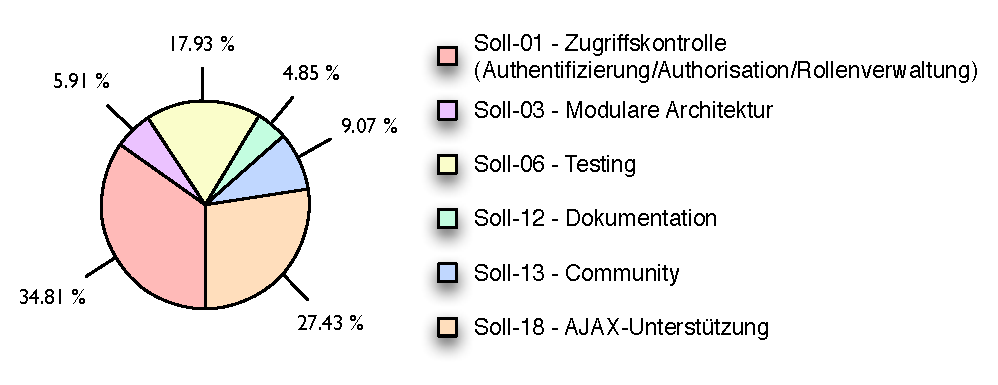
\includegraphics[width=0.95\textwidth]{./image/gewichtungSollKriterien.pdf}
      \caption{Gewichtung der Soll-Kriterien nach der Methode des AHP}
      \label{img:gewichtungSollKriterien}
    \end{center}
  \end{figure}
  
  \subsection{Bestimmen des Erfüllungsgrades}
  
  Für die Werte zur Bestimmung der Erfüllungsgrade wird die Skala der
  Erfüllungsgrade, siehe Tabelle \ref{tab:erfuellungsgrade}, verwendet. Die
  Begründung der gegebenen Punkt wird für jeden Punkt erläutert.
  
  \subsection{A-1 - ULC, Canoo RIA Suite}
  
  ULC, Canoo Ria Suite wurde aufgrund der KO-Kriterien \ref{itm:KO-18} und
  \ref{itm:KO-19} aus der Evaluation ausgeschlossen.
  
  \subsection{A-2 - Struts 1.3.10 mit ZIP-Framework}
  
  Für Informationen zum Framework Struts 1.3.10 in Kombination mit dem \ac{ZIP}
  Framework habe ich Marco Spörri interviewt. Er arbeitet seit längerer Zeit
  damit. Struts 1.3.10 ist ein Open Source Framework, das von der Apache
  Software Foundation gepflegt wird. Der \ac{ZIP} Teil ist eine Erweiterung,
  welche in der \ac{ZKB} entwickelt wurde. Marco Spörri gehört zu den Personen,
  welche aktuell daran Erweiterungen anbringt.

  Das Ergebnis der Nutzwertanalyse ist in der Tabelle
  \ref{tab:nwaA2} ersichtlich. Der Nutzwert liegt bei 3.9829 und ist somit
  durchschnittlich, das entspricht dem Erfüllungsgrad
  \begin{itshape}mittel\end{itshape}.
  
  \begin{table}[ht]
    \sffamily 
    \begin{center}
      \begin{tabular}{r|rrr}
        \toprule
        \textbf{Kriterium} & \textbf{Gewichtung \(g\)} & \textbf{Erfüllungsgrad
        \(e\)} & \textbf{Wertigkeit \(_A-_2\)} \\
        \midrule
        Soll-01   & 34.81 \% & 6 & 2.0886 \\
        Soll-03   &  5.91 \% & 5 & 0.2955 \\
        Soll-06   & 17.93 \% & 5 & 0.8965 \\
        Soll-12   &  4.85 \% & 7 & 0.3395 \\
        Soll-13   &  9.07 \% & 4 & 0.3628 \\
        Soll-18   & 27.43 \% & 0 & 0.0 \\
        \midrule
        \midrule
        Ergebnis  & 100.00 \% &   & 3.9829 \\
        \bottomrule
      \end{tabular}
      \caption{Nutzwertanalyse der Alternative A-2 - Struts 1.3.10 mit
      ZIP-Framework}
      \label{tab:nwaA2}
    \end{center}
  \end{table}
    
  \subsubsection{Soll-01 - Zugriffskontrolle - 6 Punkte}
  
  Sowohl Struts, wie auch \ac{ZIP} bietet von Grund auf kein Rollenkonzept an.
  
  Die Authentifizierung wird ganz normal über eine Session-ID gelöst.
  
  Die Autorisierung für alle Business relevanten Requests wird vom
  Businesslayer jedes mal geprüft.
  
  Cross-Site Scripting wird über Escaping verhindert. Zudem werden alle
  Formulardaten validiert und verifiziert, somit wird SQL-Injection unterbunden.
  
  Ein Mechanismus des \ac{ZIP} Frameworks lässt alle Namen der
  \ac{HTML}-Formular Felder obfuskieren. Damit wird erreicht, dass aufgrund
  der Daten, welche vom Browser an den Server gesendet werden, nicht direkt
  auf die Businessfunktion zurückgeschlossen werden kann. Das Obfuskieren der
  Formularfelder Namen passiert bei jedem Aufbau einer HTML Seite von neuem. Das
  Mapping zwischen den generierten Namen und den jeweiligen Businessfunktionen
  wird auf dem Server gehalten.
  
  Die gängigsten Sicherheitsvorkehrungen können getroffen werden, leider bietet
  das Framework kein Rollenkonzept an, somit gibt es sechs Punkte
  
  \subsubsection{Soll-03 - Modulare Architektur - 5 Punkte}
  
  Es steht kein Add-On oder Plugin Mechanismus zur Verfügung. Da
  \ac{JSP}\footnote{JavaServer Pages, abgekürzt JSP, ist eine von Sun
  Microsystems entwickelte Web-Programmiersprache. Sie erlaubt, Java-Code und
  spezielle JSP-Aktionen in HTML- oder XML-Seiten einzubetten, siehe
  \cite{JavaServerPages}.} für die View verwendet wird, kann durch die
  Erweiterung von Tag-Bibliotheken\footnote{Tag-Bibliotheken sind ein
  Bestandteil der JSP-Spezifikation. Mit ihrer Hilfe ist es möglich, JSP-Seiten
  zu entwickeln, die nur noch wenig bis gar keinen Java-Code beinhalten, siehe
  \cite{TagLibrary}} ein modularer Ansatz verfolgt werden. Neu entwickelte
  Tag's werden im ZIP-Framework integriert und so für zukünftige Verwendung
  zentral verwaltet.
  
  \ac{JSP} biete mit dem \(<jsp:include>\) Tag die Möglichkeit eines modularen
  Ansatzes für die Softwareentwicklung. Jedoch ist die Trennung zwischen Model,
  View und Controller bei JSP-Files meistens nicht sehr klar, was nicht gerade
  im Sinne einer modularen Architektur ist.
  
  Wie überall in der Javawelt kann durch die Einbindung von
  JAR-Dateien\footnote{Ein Java Archive (umgangssprachlich aufgrund der
  Dateiendung auch JAR-Datei genannt) ist eine ZIP-Datei. JARs werden vor allem
  zur Verteilung von Java-Klassenbibliotheken und -Programmen eingesetzt, siehe
  \cite{JARDatei}} die Funktionalität des Frameworks erweitert werden.
  
  Durch den modularen Ansatz mit Tag-Bibliotheken gibt es fünf Punkte.
  
  \subsubsection{Soll-06 - Testing - 5 Punkte}
  
  Struts 1.3.10 biete grundsätzlich die Unterstützt für Unit Tests. Die
  Notwendigen Klassen befinden sich im Package \(org.apache.struts.mock\).
  
  Für das Testen von Views gibt es keine Komponenten, deshalb muss auf Tools
  von Drittanbieter, wie zum Beispiel Selenium, zurückgegriffen werden.
  
  Durch die Unterstützung von Unit Tests gibts 5 Punkte.
  
  \subsubsection{Soll-12 - Dokumentation - 7 Punkte}
  
  Das Projekt Struts 1.3.10 bietet Dokumentation in der Form von JavaDoc, ein
  FAQ und HowTo. Zudem werden Links zu FAQ's und HowTo's von Drittparteien
  aufgelistet. Es gibt ein User Guide in dem alle Funktionen beschrieben werden.
  
  Auf Amazon gibt es eine Fülle von Büchern welche sich direkt mit Struts oder
  indirekt mit \ac{JSP} befassen.
  
  Für das \ac{ZIP}-Framework existiert die Dokumentation der API, via JavaDoc.
  Es existiert ein Tutorial Projekt, in welchem die möglichen Funktionen
  implementiert sind. Zusätzlich gibt es eine Dokumentation die in Text
  verfasst wurde und es existiert eine Präsentationsreihe, auf der Basis von
  PowerPoint, die zu Schulungszecken erstellt wurde.
  
  Für das Framework existiert insgesamt eine solide Dokumentation somit gibt es
  sieben Punkte.
  
  \subsubsection{Soll-13 - Community - 4 Punkte}
  
  Apache Struts 1.x wurde im Jahre 2000 ins Leben gerufen und hat somit schon
  einige Jahre auf dem Buckel. Die aktuell stabile Version ist 1.3.10. Mit dem
  Java Web Framework Struts 2 wurde die Nachfolgerin ins Leben gerufen, welche
  aktuell in der Version 2.2.3 verfügbar ist.
  
  Laut ohloh\footnote{ohloh ist eine Community Plattform für
  Softwareentwickler, siehe \url{http://www.ohloh.net/}} gibt es 89 User, die
  Struts 1.x verwenden. Laut ohloh gibt es aktuell nur noch eine Person, welche
  das Framework aktiv weiterentwickelt. Das liegt wohl daran, dass die Version
  1.3.10 entweder sehr stabil ist, oder das die meisten Entwickler auf die 
  neuste Version von Apache Struts 2.2.3 umgestiegen sind.
  
  Für Struts 1.x gibt es keine DZone Refcard.
  
  Bei DZone findet man 9136 Posts, welche sich mit Struts 1 befassen. Dies wurde
  mit dem Suchbegriff ``Struts 1'' eruiert.
  
  Das ZIP-Framework wird von ca. 30 Personen eingesetzt und aktuell gibt es vier
  Personen, welche Bugs beheben und Features einbauen. Das Framework wurde von
  der \ac{ZKB} für eigene Zwecke entwickelt und wird auch nur innerhalb der
  \ac{ZKB} verwendet.
  
  Struts 1.x ist wohl schon länger überholt und durch Struts 2.x abgelöst
  worden. Das Zip-Framework wird aktuell noch weiterentwickelt und auch
  eingesetzt. Durch die veraltete Grundlage mit Struts 1.x gibt es nur vier
  Punkte.

  \subsubsection{Soll-18 - AJAX-Unterstützung - 0 Punkte}
  
  Apache Struts 1.3.10 und auch das ZIP-Framework bieten keine \ac{Ajax}
  Unterstützung, somit gibt es null Punkte.
  
  \subsection{A-3 - Vaadin 6.6.0}
  
  Das Ergebnis der Nutzwertanalyse ist in der Tabelle \ref{tab:nwaA3}
  ersichtlich. Der Nutzwert liegt bei 7.0168 und ist somit relativ hoch und
  entspricht dem Erfüllungsgrad \begin{itshape}gut\end{itshape}.
    
  \begin{table}[ht]
    \sffamily 
    \begin{center}
      \begin{tabular}{r|rrr}
        \toprule
        \textbf{Kriterium} & \textbf{Gewichtung \(g\)} & \textbf{Erfüllungsgrad
        \(e\)} & \textbf{Wertigkeit \(_A-_3\)} \\
        \midrule
        Soll-01   & 34.81 \% & 7 & 2.4367 \\
        Soll-03   &  5.91 \% & 5 & 0.2955 \\
        Soll-06   & 17.93 \% & 9 & 1.6137 \\
        Soll-12   &  4.85 \% & 8 & 0.3880 \\
        Soll-13   &  9.07 \% & 4 & 0.3628 \\
        Soll-18   & 27.43 \% & 7 & 1.9201 \\
        \midrule
        \midrule
        Ergebnis  & 100.00 \% &   & 7.0168 \\
        \bottomrule
      \end{tabular}
      \caption{Nutzwertanalyse der Alternative A-3 - Vaadin 6.6.0}
      \label{tab:nwaA3}
    \end{center}
  \end{table}
  
  \subsubsection{Soll-01 - Zugriffskontrolle - 7 Punkte}
  
  Vaadin biete von sich aus keine Unterstützung für Authentifizierung und
  Autorisierung an. Es gibt aber ein alternatives Projekt, das sich
  vaadin-appfoundation\footnote{Projektinformationen sind hier zu finden:
  \url{http://code.google.com/p/vaadin-appfoundation/}} nennt und im
  offiziellen Vaadin add-on Repository verfügbar ist. Dieses Projekt beinhaltet
  ein Autorisierungsmodul, mit dem ein Rollenkonzept implementiert werden kann.
  
  Zum Thema Sicherheit behauptet Vaadin von sich, derzeit eines der sichersten
  Web Frameworks zu sein.
  
  \begin{quote}
  \begin{itshape}``The server-side architecture of Vaadin is immune to the usual
  risks affecting many other RIA frameworks. Your business logic and UI state
  are kept securely on the server, and never sent to the browser where it could
  be analyzed by a potential attacker. Vaadin doesn't even trust the components
  or the RPC model of GWT, which is used to render the UI.

  In addition, we have implemented several other security mechanisms in Vaadin
  to prevent eg. man-in-the-middle and cross-site scripting
  attacks.''\end{itshape}
  \footnote{Vaadin Ltd., 2011, siehe \cite{VaadinSecurityAlerts}}
  \end{quote}
  
  Zwei Punkte Abzug, da keine Rollenverwaltung von Grund auf vorhanden ist.
  
  \subsubsection{Soll-03 - Modulare Architektur - 5 Punkte}
  
  Vaadin bietet ein eigenes Add-on Repository an, unter welchem Erweiterungen
  zum Framework bezogen werden können. Das deutet auf eine modulare Architektur
  hin.
  
  Es können eigene \ac{GUI} Komponenten erstellt und auch einfach
  wiederverwendet werden. Dafür verwendet Vaadin den modularen Aufbau von
  \ac{GWT}.
  
  Wie modular die Architektur wirklich ist, konnte ich nach meinem Research
  nicht genau abschätzen, deshalb gibt es nur fünf Punkte.
  
  \subsubsection{Soll-06 - Testing - 9 Punkte}
  
  Für das Framework steht eine komplette Test Suite namens TestBench zur
  Verfügung. Mit TestBench können UI Regressionstest aufgezeichnet und
  automatisiert durchgeführt werden. TestBench ist eine kostenpflichtige
  Extension zu Vaadin. Das ganze basiert auf Selenium, einem Open Source
  Projekt zur Abwicklung von Tests im Web-Umfeld, und JUnit, einem Open Source
  Projekt zur Abbildung von Unit Tests.
  
  Da ein Test Framework existiert, das auf aktuellen Techniken basiert, gibt es
  die maximale Punktzahl.
  
  \subsubsection{Soll-12 - Dokumentation - 8 Punkte}
  
  Die Entwickler haben sogleich ein komplettes Buch zum Framework mit vielen
  hilfreichen Beispielen geschrieben, siehe \cite{BookOfVaadin}. Das Buch ist
  in \ac{HTML} oder als \ac{PDF} frei verfügbar und kostenlos. Es enthält alle
  wichtigen Informationen, welche zur Entwicklung nötig sind. Auf
  Amazone\footnote{Amazon ist ein online Buchladen, siehe
  \url{http://www.amazon.de}} gibt es nur ein weiteres Buch, das sich diesem
  Framework gewidmet hat, das ist aber nicht weiter schlimm, da das Framework
  relativ neu ist.
  
  Die Dokumentation wird auf der Webseite mit einer Menge von Tutorials
  abgerundet. Es existieren auch die üblichen Dinge, wie das JavaDoc zum
  \ac{API}, die Hinweise auf die Lizenz, \ac{FAQ} und vieles mehr. Das alles
  wirk sehr sauber, schön und vollständig.
  
  Leider existiert die Dokumentation nur auf Englisch, deshalb gibt es einen
  Punkt Abzug.
  
  \subsubsection{Soll-13 - Community - 4 Punkte}
  
  Das Framework Vaadin ist unter seinem Namen noch nicht sehr lange bekannt,
  früher wurde es unter dem Namen IT Mill entwickelt. Das kann zu einem leicht
  falschen Resultat führen, wenn man die Community nach Vaadin untersucht.
  
  Laut ohloh\footnote{ohloh ist eine Community Plattform für
  Softwareentwickler, siehe \url{http://www.ohloh.net/}} gibt es 183 User, die
  Vaadin verwenden und 62 Contributer. Die meisten Commits werden von den
  Mitarbeitern der Firma Vaadin Ltd gemacht, welche das Framework
  erfunden hat.
  
  Bei DZone\footnote{Eine Community Plattform für Softwareentwickler, welche
  unter dem Namen ``Javalobby - The heart of the Java developer community''
  einen speziellen Bereich für Java Entwickler hat, siehe
  \url{http://www.dzone.com/}} findet man 75 Posts, welche sich direkt mit
  Vaadin befassen. Dies wurde mit dem Suchbegriff ``Vaadin'' eruiert.
  
  Für Vaadin gibt es ein DZone Refcard\footnote{Sogenannte Cheat Sheets, die
  meistens von den Entwicklern eines Frameworks selbst verfasst werden. Sie
  stehen gratis unter der \ac{URL} \url{http://refcardz.dzone.com/} zur
  Verfügung.}. Wenn für ein Framework ein Refcard existiert, sagt das aus, dass
  es von der Community verwendet wird.
  
  Die Firma Vaadin Ltd bietet mit Vaadin Pro die Möglichkeit von bug-fix
  priority, direkten Support durch das Vaadin Entwicklungsteam und Zugriff auf
  eine Vaadin Knowledge-Base, siehe \cite{VaadinPro}. Zudem können gegen ein
  Entgeld Fachkräfte für einen Tag oder drei Wochen (ein Sprint im Sinne von
  Scrum) verpflichtet werden. Es gibt auch die Möglichkeit einen Proof of
  Concept durch das Vaadin Entwicklungsteam erstellen zu lassen.
  
  Der Support durch die Firma Vaadin Ltd sieht sehr gut aus, die Community für
  Vaadin ist aber gerade erst dabei sich zu bilden und noch nicht sehr stark, somit
  sind es nur 4 Punkte.

  \subsubsection{Soll-18 - AJAX-Unterstützung - 7 Punkte}
  
  \ac{Ajax} wird massiv unterstützt. Alle \ac{UI} Komponenten und deren
  Aktionen, sowie auch das ganze Layout Management basieren auf diesem Prinzip.
  Das Programmiermodell sieht vor, dass der Entwickler die komplette
  Funktionalität in Java entwickeln kann, sodass das Framework alle dafür
  notwendigen Javascripts, \ac{HTML} und \ac{CSS} generiert. Zudem kann
  eine zusätzliche Javascript Library wie JQuery oder Prototype in die
  Applikation integriert werden.
  
  Leider können Vaadin Applikationen nicht auf die Verwendung von Java
  Script verzichten. Wenn Java Script im Browser nicht unterstützt oder
  deaktiviert ist, können Vaadin Applikationen nicht ausgeführt werden. Durch
  das fehlen einer Fallback-Lösung gibt es zwei Punkte Abzug.
  
  \subsection{A-4 - Apache Wicket 1.4.17}
  
  Um an wertvolle Informationen über Apache Wicket zu kommen, habe ich Stefan
  Pudig interviewt. Er hatte schon ein Projekt in Apache Wicket implementiert,
  und kennt sich im allgemeinen mit der Materie aus. Zudem wurde das Buch
  ``Wicket - Komponentenbasierte Webanwendungen im Java'', siehe \cite{Wicket} als
  Referenz verwendet.
  
  Das Ergebnis der Nutzwertanalyse ist in der Tabelle \ref{tab:nwaA4}
  ersichtlich. Der Nutzwert liegt bei 6.4282 und sagt aus, dass das Framework
  dem Erfüllungsgrad \begin{itshape}gut\end{itshape} entspricht.
  \newline
  
  \begin{table}[ht]
    \sffamily 
    \begin{center}
      \begin{tabular}{r|rrr}
        \toprule
        \textbf{Kriterium} & \textbf{Gewichtung \(g\)} & \textbf{Erfüllungsgrad
        \(e\)} & \textbf{Wertigkeit \(_A-_4\)} \\
        \midrule
        Soll-01   & 34.81 \% & 7 & 2.4367 \\
        Soll-03   &  5.91 \% & 5 & 0.2955 \\
        Soll-06   & 17.93 \% & 6 & 1.0758 \\
        Soll-12   &  4.85 \% & 7 & 0.3395 \\
        Soll-13   &  9.07 \% & 7 & 0.6349 \\
        Soll-18   & 27.43 \% & 6 & 1.6458 \\
        \midrule
        \midrule
        Ergebnis  & 100.00 \% &   & 6.4282 \\
        \bottomrule
      \end{tabular}
      \caption{Nutzwertanalyse der Alternative A-4 - Apache Wicket 1.4.17}
      \label{tab:nwaA4}
    \end{center}
  \end{table}
  
  \subsubsection{Soll-01 - Zugriffskontrolle - 7 Punkte}
  
  Es existieren folgende Securityfeatures, welche von Grund auf dabei sind:
  
  \begin{itemize}
    \item Wenn über HTTPS kommuniziert wird, wird ein Session Hijacking
    unterbunden, sofern kein Zugriff auf die Server Komponente, in der Apache
    Wicket läuft, besteht.
    \item Cross-Site Scripting wird anhand einer Escaping
    Funktion\footnote{Hierunter versteht man ein Maskierten der
    JavaScript-Funktionszeichen, sodass diese nicht ausgeführt, sondern
    angezeigt werden, siehe \cite{Wicket} S. 299} verhindert.
    \item SQL-Injection wird ebenfalls anhand eines Escapings unterbunden. Zudem
    wird einem geraten in Java mit \(PreparedStatements\) zu arbeiten, damit
    übergebene Parameter nicht mehr interpretiert werden, siehe \cite{Wicket} S.
    299.
    \item Authentifizierung und Autorisierung Mechanismen werden vom Framework
    nur grundlegend unterstützt. 
    \item Ein Rollenkonzept wird von Grund auf nicht angeboten, dafür gibt es
    ein zusätzliches Framework namens ``Wicket Auth Roles''. 
  \end{itemize}
  
  \noindent
  Zwei Punkte Abzug, da keine Rollenverwaltung von Grund auf vorhanden ist.
  
  \subsubsection{Soll-03 - Modulare Architektur - 5 Punkte}
  
  Bei diesem Punkt stütze ich mich auf die Aussagen von Stefan Pudig.
  
  Ein offizielles Add-on oder Plugin Repository existiert nicht für Apache
  Wicket. Dafür können zusätzliche Features in der Form von Bibliotheken manuell
  zum Projekt hinzugefügt werden. Zudem wird eine Maven Integration
  gewährleistet.
  
  Die Erweiterung von Komponenten des grafischen User Interfaces (UI) wird sehr
  gut unterstützt. Durch die Fähigkeit des Vererbens können Komponenten einfach
  abgeleitet und verändert werden. Diese können dann auch einfach
  wiederverwendet werden.
  
  Wie modular das Framework selber ist, konnte Stefan Pudig mir nicht nennen, er
  meint aber, dass die meisten Business Applikationen mit den bestehenden
  Komponenten abgebildet werden können.
  
  Durch das fehlen eines Add-on Repositories gibt es nur fünf Punkte.
  
  \subsubsection{Soll-06 - Testing - 6 Punkte}
  
  Wicket bietet eine \ac{API} an, mit welcher Unit Tests durchgeführt werden
  können. Es können damit alle gängigen funktionalitäten des Frameworks
  getestet werden, siehe \cite{Wicket} S. 255ff. Dafür muss die Applikation
  nicht deployed werden, sondern die Applikation wird direkt instanziiert.
  
  Leider wird kein Möglichkeit geboten, Regressionstests abzubilden. Dafür muss
  man auf auf bestehende Lösungen, wie
  Selenium\footnote{Siehe \url{http://www.seleniumhq.org/} oder
  \url{http://code.google.com/p/webdriver}} zurückgreifen.
  
  Da von Grund auf keine Regressionstests möglich sind gibt es nur sechs Punkte
  
  \subsubsection{Soll-12 - Dokumentation - 7 Punkte}

  Auf Amazon werden fünf Bücher zum Apache Wicket Framework
  angeboten. Das sind genug Referenzen, um sich in die Thematik tief
  einzuarbeiten.
  
  Die Projektseite\footnote{Apache Wicket Projektseite, siehe
  \url{http://wicket.apache.org/}} ist schlicht und übersichtlich, wie man das
  von Apache Projekten gewohnt ist. Es ist das JavaDoc zum \ac{API} verfügbar,
  es gibt eine Handvoll Beispiele, und eine Übersicht zu den unterstützten
  Komponenten, zudem gibt es eine komplette Dokumentation zum Thema Wicket. Ein
  paar Links, zu Blogs, die sich mit der Materie befassen, werden auch
  propagiert.
  
  Eine unumgängliche Erweiterung der Dokumentation ist das offizielle
  Wiki\footnote{Siehe \url{https://cwiki.apache.org/WICKET/}}. Hier werden alle
  notwendigen Informationen und Tips und Tricks zusammengezogen.
  
  Alles in allem ist der Umfang gut, die erwähnten Bereiche sind aber nur in
  Englisch verfügbar. Zudem wirkt die Dokumentation eher wie zusammengewürfelt.
  Deshalb gibt es zwei Punkte Abzug.
 
  \subsubsection{Soll-13 - Community - 7 Punkte}
  
  Wicket existiert seit dem Jahr 2004, siehe \cite{WikiWicket}.

  Laut ohloh gibt es 119 User, die Apache Wicket verwenden und 42 Contributer.

  Bei DZone findet man 546 Posts, welche sich direkt, oder eventuell auch
  indirekt, mit Apache Wicket befassen.

  Für Apache Wicket gibt es eine DZone Refcard.
  
  Durch das sich Apache Wicket nun schon über sieben Jahre im Java Web Framework
  Zirkus halten konnte und es immer noch eine aktive Community gibt, werden
  sieben Punkte erteilt.
  
  \subsubsection{Soll-18 - AJAX-Unterstützung - 6 Punkte}
  
  Wicket bietet eine AJAX Unterstützung an, bei der die Funktionalität komplett
  in Java entwickelt werden kann. Die dafür notwendigen Javascripts, welche die
  Funktionalität bieten, werden durch das Framework generiert.
  
  Leider werden nur eine begrenzte Anzahl von Komponenten angeboten, welche
  via \ac{Ajax} an Funktionalität gewinnen. Es handelt sich dabei um bekannte
  Anwendungsfälle, wie: Formvalidierung, Paging navigation, Panel lazy loading
  oder TextField autocomplete. Es gibt noch ein paar weitere Szenarien,
  die ich hier nicht erwähnt habe. Zudem kann eine zusätzliche Javascript
  Library wie JQuery oder Prototype in die Applikation integriert werden, um
  damit das \ac{GUI} aufzuwerten.
  
  Wicket bietet eine Fallback Strategie für gewisse Komponenten. Damit wird die
  Funktionalität auch bei fehlender Javascript Unterstützung gewährleistet.
  
  Durch die begrenzte Unterstützung von Komponenten gibt es nur sechs Punkte

  \section{Resultat}
  
  Die Evaluation ist knapp ausgegangen, zumindest auf dem vordersten zwei
  Plätzen. Da hat ``A-3 - Vaadin 6.6.0'' gegenüber ``A-4 - Apache Wicket
  1.4.17'' den leicht höheren Nutzwert erreicht.
  
  Das Java Web Framework ``A-2 - Struts 1.3.10 mit ZIP-Framework'', welches
  aktuell von der IT-Architektur als der Standard vorgeschrieben wird, hat nur
  mittelmässig abgeschnitten.

  Das Framework ``A-1 - ULC, Canoo RIA Suite'' ist leider aufgrund der
  KO-Kriterien aus der Evaluation ausgeschlossen worden.
  
  Das Endergebnis wird in der Tabelle \ref{tab:ergebnisDerEvaluation} in Form
  einer Rangliste zusammenfassend dargestellt.
  \newline
  
  \begin{table}[ht]
    \sffamily 
    \begin{center}
      \begin{tabular}{clr}
        \toprule
        \textbf{Rang} & \textbf{Java Web Framework} & \textbf{Nutzwert} \\
        \midrule
        1 & A-3 - Vaadin 6.6.0 & 7.0168 \\
        2 & A-4 - Apache Wicket 1.4.17 & 6.4282 \\
        3 & A-2 - Struts 1.3.10 mit ZIP-Framework & 3.9829 \\
        - & A-1 - ULC, Canoo RIA Suite & --- \\
        \bottomrule
      \end{tabular}
      \caption{Ergebnis der Evaluation als Rangliste.}
      \label{tab:ergebnisDerEvaluation}
    \end{center}
  \end{table}
